The function \textit{ScenarioLoading} takes as input such scenario.mat file and generate the map X and Y coordinates useful for reference tracking merging all the pieces of road that compose the whole scenario.

The sections Simulation and Reference Signal defines the time span for the simulation and initialise the vectors to allocate all the map waypoints and car orientation, after the function \textit{reference\_generator} up-sample the map according to the prediction horizon and the vehicle speed generating a map with higher density of points to optimize the path following algorithm.









The script named \textit{MPC\_controller} contains the code required to launch the MPC algorithm.
The first line of code initialise the controller defining all the parameters needed for its execution and the reference trajectory that the path planner will follow.

The function \textit{loadParameters} takes as input the vehicle ID, an integer from 1 to 5 that is used as selector for car data as shown in Table \ref{tab:vehicle_data}.

Assuming that the car is already traveling at a speed \textit{V}, the initial conditions for the other states and for the two inputs are all set equal to zero.


next the function \textit{odometer} compute the total distance covered by the car following the scenario in order to let the simulation terminates exactly when the road ends.

A few lines of code are used to create a discrete time state space model for the plant and assign the value for the prediction and control horizon as well as the weights of the output and manipulated variables.

In the successive section of code are defined the constraint matrices, which correctly tuned, guarantee that the vehicle follows the reference without going off the road  i.e. stays within the lane width limits and is capable to avoid an obstacle when is inside the sensors detection range.



\subsection{seconda parte} % ALE
Finally, the last section in the main script is the one where the simulation actually occurs. At each time$-$step, different instructions are repeated in a \textit{for} loop to simulate the controller in a closed$-$loop fashion.\\
First, the current state and the inputs are used in the function \textit{obstacleVehicleModelDT} to generate a discrete$-$time model, using the Zero$-$Order Hold (ZOH) method, and consequently to generate the nominal conditions for the discrete plant and the measurements. Then, the reference path is updated: starting from an index that is increased at each cycle, the trajectory data are read along the prediction horizon length. Once the new plant model and nominal conditions are calculated, they are used as inputs for the \textit{mpcmoveAdaptive} Matlab command that computes the Adaptive MPC control action at current time. This same control action is subsequently used as input to the \textit{VehicleModelCT\_DYN\_ode} function that outputs the differential equations relative to the vehicle dynamic model; these equations are integrated from 0 to the time$-$step using the \textit{ode45} function. In the end, the loop is concluded assigning to the next state\footnote{The \textit{next} state in the current cycle will correspond to the \textit{current} state in the successive cycle as the index is increased} the result of the integration.\\
The pattern described above is repeated \textit{n} times, where \textit{n} represent the ratio between the set simulation duration and resolution.

\subsection{MPC Algorithm}  
Once the controller has been initialised, all is set to begin the simulation.\\
% \\At each time$-$step, different instructions are repeated in a \textit{for} loop to simulate the controller in a closed$-$loop fashion. 
% Figure \ref{fig:MPC_scheme} graphically shows the general concept behind a model predictive control; below it is described the MATLAB algorithm that follows the same scheme.
% \begin{figure}[H]
%     \centering
%     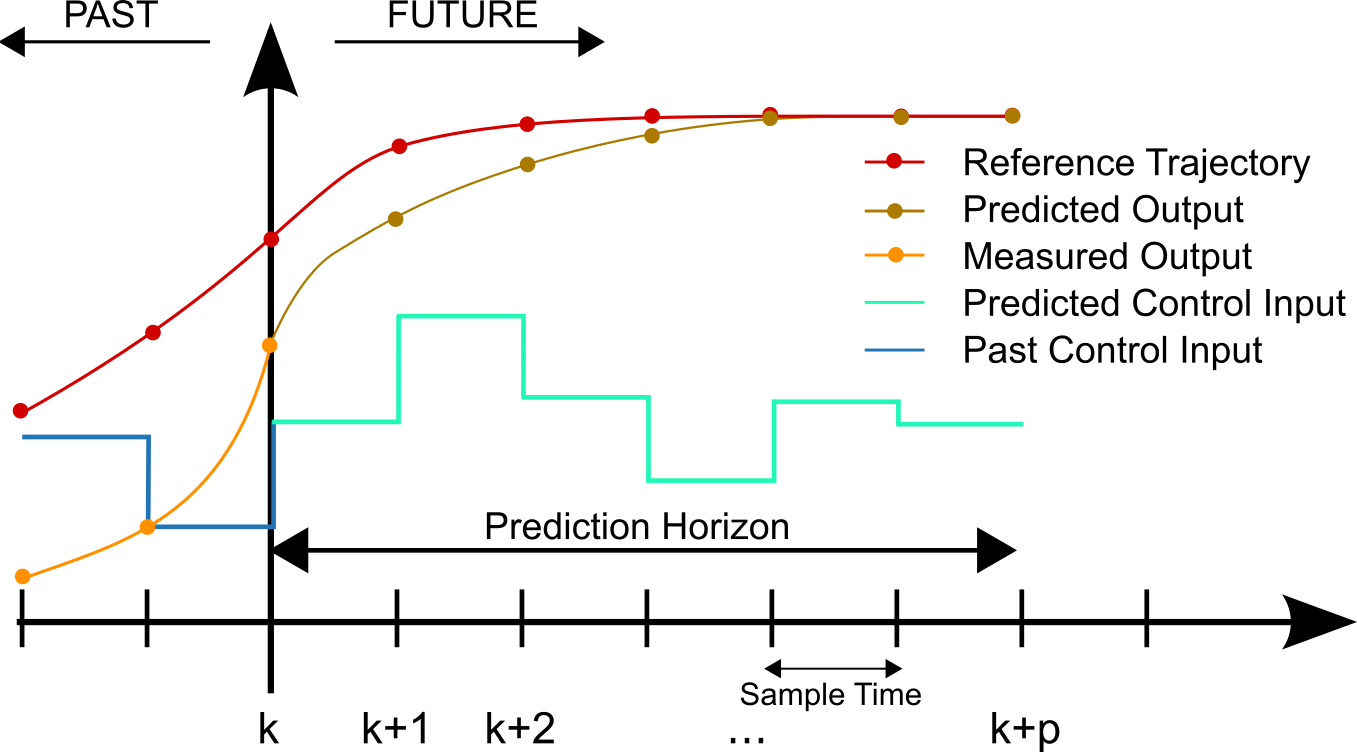
\includegraphics[width=0.9\textwidth]{Figures/MPC_scheme_basic.png}
%     \caption{MPC algorithm scheme}
%     \label{fig:MPC_scheme}
% \end{figure}
First, the current state and the inputs are used in the function \textit{obstacleVehicleModelDT} to generate a discrete$-$time model, using the Zero$-$Order Hold (ZOH) method, and consequently to generate the nominal conditions for the discrete plant and the measurements. Then, the reference path is updated: starting from an index that is increased at each cycle, the trajectory data are read along the prediction horizon length. Once the new plant model and nominal conditions are calculated, they are used as inputs for the \textit{mpcmoveAdaptive} MATLAB command that computes the Adaptive MPC control action at current time. This same control action is subsequently used as input to the \textit{VehicleModelCT\_DYN\_ode} function that outputs the differential equations relative to the vehicle dynamic model; these equations are integrated from 0 to the time$-$step using the \textit{ode45} function.
\\In the end, the loop is concluded assigning to the next state\footnote{The \textit{next} state in the current cycle will correspond to the \textit{current} state in the successive cycle as the index is increased} the result of the integration.\\
The pattern described above is repeated \textit{n} times, where \textit{n} represent the ratio between the set simulation duration and resolution.

